\documentclass[11pt,a4paper]{article}
\usepackage[top=14mm,bottom=14mm,left=18mm,right=18mm]{geometry}
\usepackage{fontspec}
\setmainfont{Liberation Serif}
\setsansfont{NimbusSans-Regular.otf}[BoldFont={NimbusSans-Bold.otf},ItalicFont={NimbusSans-Italic.otf},BoldItalicFont={NimbusSans-BoldItalic.otf}]
\usepackage{amsmath,amssymb,mathtools}
\usepackage{unicode-math}
\setmathfont{Latin Modern Math}
\usepackage{xcolor,tikz}
\usepackage[skins]{tcolorbox}
\usepackage{microtype}
\usepackage[hidelinks]{hyperref}
\definecolor{ink}{HTML}{192B3A}
\definecolor{muted}{HTML}{53636B}
\definecolor{blue}{HTML}{264B6B}
\definecolor{teal}{HTML}{167571}
\definecolor{pale}{HTML}{F0F5F5}
\definecolor{rulegray}{HTML}{CED8DB}
\pagestyle{empty}
\setlength{\parindent}{0pt}
\setlength{\parskip}{2pt}
\setlength{\emergencystretch}{1.5em}
\setlength{\abovedisplayskip}{5pt plus 1pt minus 1pt}
\setlength{\belowdisplayskip}{5pt plus 1pt minus 1pt}
\setlength{\abovedisplayshortskip}{3pt}
\setlength{\belowdisplayshortskip}{4pt}
\newcommand{\R}{\mathbb R}
\newcommand{\Z}{\mathbb Z}
\newcommand{\F}{\mathbb F_2}
\newcommand{\rank}{\operatorname{rank}}
\newcommand{\blockheading}[2]{\par\vspace{5pt}{\sffamily\bfseries\fontsize{9}{11}\selectfont\color{teal}#1}\hspace{7pt}{\bfseries\fontsize{12}{14}\selectfont\color{ink}#2}\par\vspace{1pt}}
\hypersetup{pdftitle={A 1.30\string^d Lower Bound for the Chromatic Number of Euclidean Space: Extended Abstract},pdfauthor={Ilya Hoffman},pdfsubject={A spherical-layer construction and a coefficient rank bound for the unit-distance chromatic number}}
\begin{document}
\color{ink}
\fontsize{11}{13.1}\selectfont
{\sffamily\bfseries\fontsize{8.6}{10}\selectfont\color{teal}EXTENDED ABSTRACT}\hfill
{\sffamily\fontsize{8.6}{10}\selectfont\color{muted}DISCRETE GEOMETRY}
\par\vspace{3pt}{\color{teal}\hrule height 0.7pt}\vspace{8pt}
{\fontsize{23}{25.5}\selectfont\bfseries
A $1.30^d$ Lower Bound for the\\
Chromatic Number of Euclidean Space\par}
\vspace{5pt}
{\bfseries Ilya Hoffman}\quad
{\fontsize{10}{12}\selectfont\href{mailto:ilya.hoffman@gmail.com}{ilya.hoffman@gmail.com}}\hfill
{\sffamily\fontsize{8.5}{10}\selectfont\color{muted}\href{https://orcid.org/0009-0008-9083-2105}{ORCID 0009-0008-9083-2105}}
\par\vspace{7pt}

\begin{tcolorbox}[enhanced,sharp corners,boxrule=0pt,colback=pale,
 borderline west={2pt}{0pt}{teal},left=10pt,right=10pt,top=7pt,bottom=7pt,
 boxsep=0pt,before skip=0pt,after skip=3pt]
{\sffamily\bfseries\fontsize{8.4}{10}\selectfont\color{teal}THE RESULT}\hfill
{\sffamily\fontsize{8.4}{10}\selectfont\color{muted}ORDINARY UNIT-DISTANCE COLOURING}
\par\vspace{3pt}
For an absolute constant $c>0$ and all sufficiently large $d$,
\vspace{-1pt}
{\fontsize{14.5}{17}\selectfont
\[
\chi(\R^d)\ge c\,C_*^d,
\qquad 1.309251<C_*<1.309252.
\]}
In particular, $\chi(\R^d)\ge1.30^d$ eventually. For infinitely many dimensions,
the same construction gives $\chi(\R^d)\ge1.316^d$.
\end{tcolorbox}

\blockheading{01}{The geometric idea}
For $Q=6$ or $7$, let $\mathcal A_Q$ consist of the first $Q$ entries of
$(0,1,-1,2,-2,3,-3)$. For a power of two $P\ge2$, take the entire layer
\[
V=\left\{x\in\mathcal A_Q^n:\ \sum_{i=1}^n(2x_i^2-x_i)=2P-1\right\}.
\]
Its points lie on a sphere about $o=(1/4,\ldots,1/4)$. Their midpoints lie in
$(\tfrac12\Z)^n$, at squared distance at least $n/16$ from $o$.
The parallelogram identity and parity give
\[
\rho(x,y):=\tfrac12\|x-y\|^2\in\{0,\ldots,2P-1\}.
\]
Joining pairs with $\rho=P$ gives a unit-distance graph after scaling.

\blockheading{02}{From geometry to a rank bound}
Over $\F$, the matrix $\mathcal M_{xy}=\binom{\rho(x,y)-1}{P-1}$ is one exactly
on the diagonal and the edges, with $\binom{-1}{P-1}=(-1)^{P-1}$.
Every independent set therefore indexes an identity matrix.
Newton interpolation exposes powers of a formal variable; coefficient extraction
then reduces the rank estimate to a sum of outer products. For $V\ne\varnothing$, this yields
\[
\chi(\R^n)\ge\frac{|V|}{\rank_{\F}\mathcal M}
\ge\frac{[t^{2P-1}]A_Q(t)^n}
{[s^{P-1}]\bigl(E_Q(s)^n/(1-s)^2\bigr)}.
\]
Here $A_Q(t)=\sum_{0\le j<Q}t^{j(j+1)/2}$, $E_Q(s)=\sum_{0\le j<Q}s^{e_j}$, and
$(e_0,\ldots,e_6)=(0,1,3,4,8,9,11)$; brackets denote coefficient extraction.

\blockheading{03}{A constant prefactor, uniformly in the dimension}
An elementary binomial estimate gives matching $n^{-1/2}$ factors in the vertex
count and rank bound; these cancel. The least power of two $P\ge a_*n$,
where $a_*\approx0.37198$, gives $P/n\in[a_*,2a_*)$.
Four concave lower bounds for the logarithmic rate cover this interval
using six or seven coordinate values.

\vspace{4pt}
\begin{center}
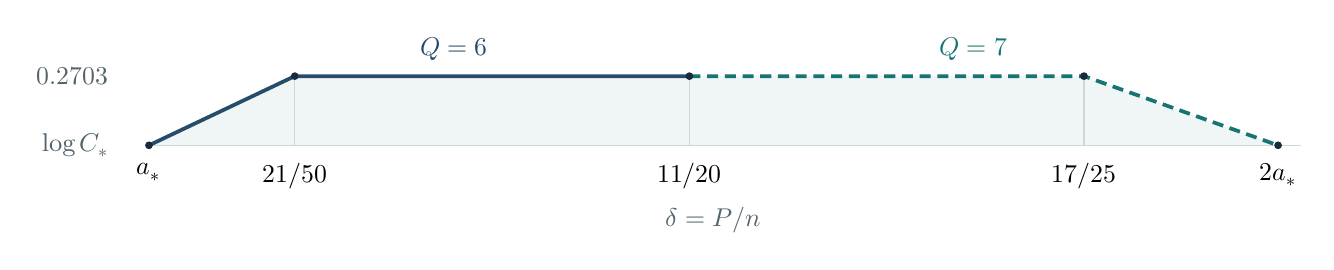
\begin{tikzpicture}[x=408pt,y=25pt,every node/.style={font=\fontsize{9.3}{10.5}\selectfont}]
\pgfmathsetmacro{\xa}{(0.42-0.3719795)/0.3719795}
\pgfmathsetmacro{\xb}{(0.55-0.3719795)/0.3719795}
\pgfmathsetmacro{\xc}{(0.68-0.3719795)/0.3719795}
\fill[pale] (0,0)--(\xa,1)--(\xc,1)--(1,0)--cycle;
\draw[rulegray,line width=.55pt] (0,0)--(1.02,0);
\foreach \x in {\xa,\xb,\xc}{\draw[rulegray,line width=.4pt] (\x,0)--(\x,1);}
\draw[blue,line width=1.35pt] (0,0)--(\xa,1)--(\xb,1);
\draw[teal,line width=1.35pt,dash pattern=on 4pt off 2.4pt] (\xb,1)--(\xc,1)--(1,0);
\foreach \x/\y in {0/0,\xa/1,\xb/1,\xc/1,1/0}{\fill[ink] (\x,\y) circle[radius=1.4pt];}
\node[anchor=east,text=muted] at (-.027,0) {$\log C_*$};
\node[anchor=east,text=muted] at (-.027,1) {$0.2703$};
\node[text=blue] at (.27,1.4) {$Q=6$};
\node[text=teal] at (.73,1.4) {$Q=7$};
\node[anchor=north] at (0,-.12) {$a_*$};
\node[anchor=north] at (\xa,-.12) {$21/50$};
\node[anchor=north] at (\xb,-.12) {$11/20$};
\node[anchor=north] at (\xc,-.12) {$17/25$};
\node[anchor=north] at (1,-.12) {$2a_*$};
\node[anchor=north,text=muted] at (.5,-.75) {$\delta=P/n$};
\end{tikzpicture}
\par\vspace{-1pt}
{\fontsize{9.4}{11}\selectfont\color{muted}The concave lower bounds lie above the four indicated chords.}
\end{center}
\vspace{-3pt}
{\color{rulegray}\hrule height .5pt}\vspace{4pt}
{\fontsize{9.5}{11.5}\selectfont\color{muted}
Four exact integer witnesses with common frequency denominator $M=200$ give a
short route to $1.30^d$. The full paper includes all algebraic proofs and finite
arithmetic data.\par}
\end{document}
